

\tikzset{every picture/.style={line width=0.75pt}} %set default line width to 0.75pt        

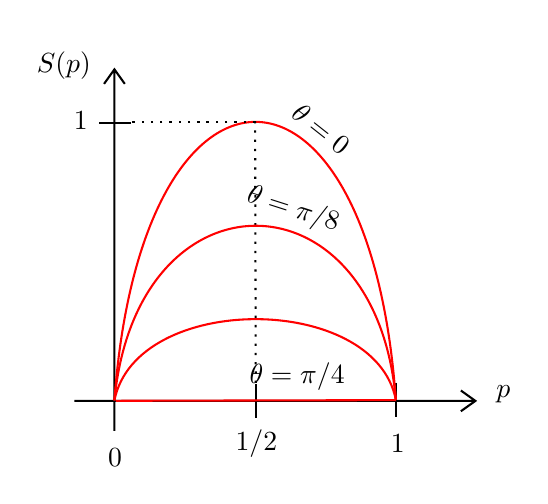
\begin{tikzpicture}[x=0.75pt,y=0.75pt,yscale=-1,xscale=1]
%uncomment if require: \path (0,300); %set diagram left start at 0, and has height of 300

%Shape: Axis 2D [id:dp5027085791119299] 
\draw  (185.02,202.37) -- (378.25,202.37)(204.34,42.64) -- (204.34,216.85) (371.25,197.37) -- (378.25,202.37) -- (371.25,207.37) (199.34,49.64) -- (204.34,42.64) -- (209.34,49.64)  ;
%Straight Lines [id:da09853418101033773] 
\draw    (339.91,193.54) -- (339.91,210.1) ;


%Straight Lines [id:da3358027007557636] 
\draw    (212.32,68.28) -- (196.98,68.28) ;


%Curve Lines [id:da3148958709948577] 
\draw [color={rgb, 255:red, 255; green, 0; blue, 0 }  ,draw opacity=1 ]   (204.34,202.13) .. controls (217.41,23.06) and (327.34,23.47) .. (339.91,201.82) ;


%Straight Lines [id:da8089499215946534] 
\draw    (272.43,194.15) -- (272.43,210.72) ;


%Straight Lines [id:da23335895135809026] 
\draw  [dash pattern={on 0.84pt off 2.51pt}]  (272.13,67.54) -- (272.43,195.99) ;


%Straight Lines [id:da42484056815365134] 
\draw  [dash pattern={on 0.84pt off 2.51pt}]  (272.13,68.03) -- (212.75,68.03) ;


%Curve Lines [id:da04941603137640582] 
\draw [color={rgb, 255:red, 255; green, 0; blue, 0 }  ,draw opacity=1 ]   (204.34,202.13) .. controls (215,89.67) and (330.33,90.33) .. (339.91,201.82) ;


%Straight Lines [id:da510763025258693] 
\draw [color={rgb, 255:red, 255; green, 0; blue, 0 }  ,draw opacity=1 ]   (340,202) -- (205,202.33) ;


%Curve Lines [id:da015065338845632326] 
\draw [color={rgb, 255:red, 255; green, 0; blue, 0 }  ,draw opacity=1 ]   (204.34,202.13) .. controls (214.75,150) and (329.75,150) .. (339.91,201.82) ;



% Text Node
\draw (391.75,199.06) node   {$p$};
% Text Node
\draw (204.65,229.73) node   {$0$};
% Text Node
\draw (340.83,222.98) node   {$1$};
% Text Node
\draw (188.09,67.17) node   {$1$};
% Text Node
\draw (272.74,222.98) node   {$1/2$};
% Text Node
\draw (292.33,190.67) node   {$\theta =\pi /4$};
% Text Node
\draw (290.5,110.17) node [rotate=-17.78]  {$\theta =\pi /8$};
% Text Node
\draw (304,71.17) node [rotate=-38.36]  {$\theta =0$};
% Text Node
\draw (180,41) node   {$S( p)$};


\end{tikzpicture}